\documentclass[titlepage, a4paper]{article}
\usepackage[english]{babel}
\usepackage[utf8]{inputenc}
\usepackage{graphicx}
\usepackage{color}
\usepackage{mathtools}
\usepackage{float}
\usepackage[parfill]{parskip}
\usepackage[margin=10pt,font=small,labelfont=bf,labelsep=endash]{caption}
\usepackage{epstopdf}
\usepackage{listings}
\epstopdfsetup{suffix=}
\DeclareGraphicsExtensions{.ps}
\DeclareGraphicsRule{.ps}{pdf}{.pdf}{`ps2pdf -dEPSCrop -dNOSAFER #1 \noexpand\OutputFile}

\lstset{literate=%
    {å}{{\r{a}}}1
    {ä}{{\"a}}1
    {ö}{{\"o}}1
    {Å}{{\r{A}}}1
    {Ä}{{\"A}}1
    {Ö}{{\"O}}1
}

\newcommand{\todo}[1] {\textbf{\textcolor{red}{#1}}}

\usepackage{fancyhdr}
\fancyhead[L]{}
\pagestyle{fancy}
\rhead{Alexander Yngve \\ Pål Kastman}
\chead{TDDC78}
\thispagestyle{empty}

\begin{document}

{\ }\vspace{45mm}

\begin{center}
  \Huge \textbf{TDDC78: Lab Report}
\end{center}
\begin{center}
  \Large Lab 3: OpenMP
\end{center}

\vspace{250pt}

\begin{center}
  \begin{tabular}{|*{3}{p{40mm}|}}
    \hline
    \textbf{Name} & \textbf{PIN} & \textbf{Email} \\ \hline
           {Alexander Yngve} & {930320-6651} & {aleyn573@student.liu.se} \\ \hline
           {Pål Kastman} & {851212-7575} & {palka285@student.liu.se} \\ \hline
  \end{tabular}
 \end{center}
\newpage

\tableofcontents
\thispagestyle{empty}
\newpage

\section{Introduction}
In this lab we were to solve a heat conducting problem on a shared memory computer, by using Open MP.

\section{Heat Conducting Problem}
In this lab we had to solve a heat conducting problem using the Jacobi iterative method.

\section{Our implementation}
When we first read the explanation of this lab, and it said that we were only allowed to use $\mathcal{O}(n)$ additional memory we started with splitting every row into equal size parts depending on how many processes we had been provided. This meant that for every row we had to synchronize so no process started on the next one before copying this area into the temporary memory. This turned out to not work good at all, instead of an decrease in time we got a heavy increase. We think that this is because the program needed to synchronize and wait for each other alot.

But then we realized that the original implementation used \textit{2N} of memory, which is still inside $\mathcal{O}(n)$. So instead we let every process have their own regions of the array, so say for instance that the array is 1000 rows and we are running 4 processes then every process will have 200 rows each. The problem here is that when the processes reaches the final row they will need values from a row that the next process already has modified, because of this we needed to use another \textit{N} of memory per process.

Every process will now use \textit{3N} of memory which will give us a total additional memory of \textit{3N * p} (where p is the no. processes), even if this sounds alot it will still be inside $\mathcal{O}(n)$ if $p \ll N$, which can be assumed since p is normally equal to the number of cores in the processor.

Every process calculates the error of every index and if the error is greater than the tolerance then we set a flag which will make the program end the initial while-loop. Only one process is allowed to update this flag at time.

\section{Execution times}


\begin{figure}[H]
  \centering
  \scalebox{0.48}{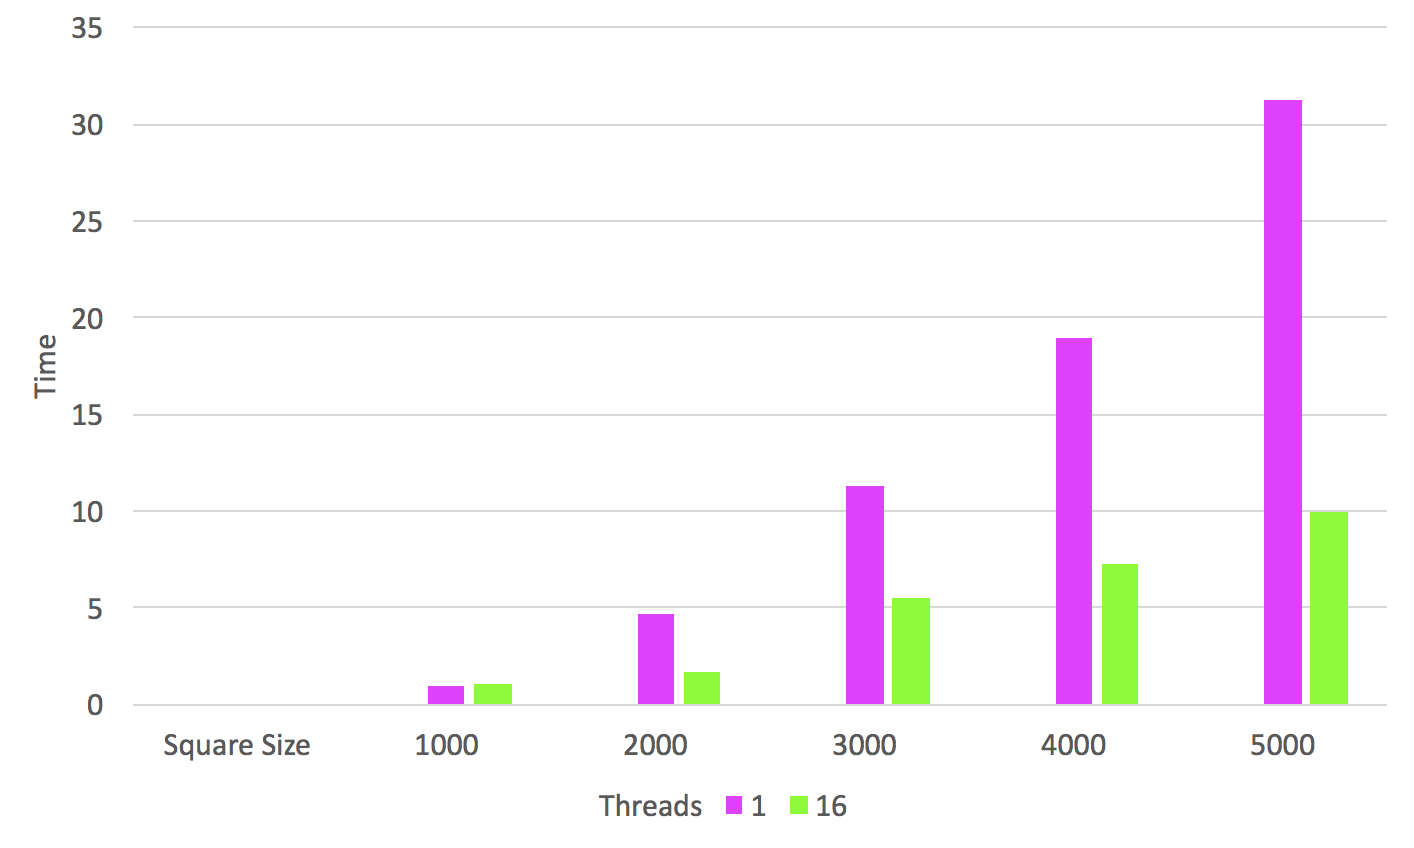
\includegraphics{img/results.png}}
  \caption{Results for different sizes of the square running on 1 and 16 threads.}
  \label{fig:results}
\end{figure}


\end{document}

%% \begin{table}[H]
%%   \centering
%%   \caption{Miss rates}
%%   \begin{tabular}{|*{3}{p{20mm}|}}
%%     \hline
%%     \textbf{Miss rates} & {test1} & {test2} \\ \hline
%%            {cache1} & {0.0091} & {0.1577} \\ \hline
%%            {cache2} & {0.0177} & {0.0235} \\ \hline
%%   \end{tabular}
%%   \label{tab:table1}
%% \end{table}


%% \begin{figure}[H]
%% 	\centering
%% 	\scalebox{0.342}{\includegraphics{img/data-cache.png}}
%% 	\caption{Only data stored in cache.}
%% 	\label{fig:data-cache}
%% \end{figure}
